\chapter{Eficiência Energética}
\section{Consumo de Energia}
\subsection{Consumo médio de energia de uma casa com família de 4 pessoas}

	De acordo com os dados coletados no Anuário Estatístico de Energia Elétrica de 2013, a média de consumo de uma residência no Distrito Federal, dos anos de 2008 à 2012, é de 217,72 kWh/mês, porém, esses dados não levam em consideração o tamanho da habitação ou a quantidade de moradores. Segundo o mesmo anuário, cada habitante gasta em média 2,1532 kWh/dia, fazendo um cálculo meramente estatístico, numa estimativa grosseira, supondo um mês com 30 dias e 4 habitantes com a média de consumo idênticas, obtemos que o consumo médio de energia de uma residência com 4 pessoas sendo de 258,384 kWh/mês. 

	Ainda de acordo com esses valores, pode-se supor que essa média não leva em consideração a classe social da família, onde, a grosso modo, sabe-se que quanto maior a renda familiar, maior serão os seus gastos. Como os equipamentos de segurança e outros objetos mais específicos voltados a automação e outros equipamentos que fogem do padrão residencial não foram bem detalhados, faz-se uma estimativa, ainda embasado no consumo médio residencial brasileiro, de que a família consumirá uma média de 500 kWh/mês.\cite{epeanuario}


\section{Fontes de Energia}

\subsection{O que são fontes renováveis?}

	As fontes de energia renováveis, são aquelas em que a sua utilização e uso 
é renovável e pode-se manter e ser aproveitado ao longo do tempo sem 
possibilidade de esgotamento dessa mesma fonte, exemplos deste tipo de 
fonte são a energia eólica e solar.\cite{suapesquisaenergiarenovavel}

\subsection{Benefícios de utilizar fontes renováveis para suprir a demanda de energia da casa}

	As energias renováveis não poluem o ambiente e tem caráter inteiramente sustentável. no geral, causam um pequeno impacto (poluição, desmatamento) ao meio ambiente. Portanto, são excelentes alternativas ao sistema energético tradicional, principalmente numa situação de luta contra a poluição atmosférica e o aquecimento global.

\subsection{Quais fontes de energia utilizar? Por quê?}

	As fontes utilizadas na casa serão solar e eólica. Por serem de produção independente, privando a residência da dependência do uso da energia elétrica fornecida pela concessionária de abastecimento. Em análise aos fatores ambientais, essas fontes se tornam bastante produtivas e de ótima escolha, pois não geram transtornos para os habitantes da casa e minimizam custos com manutenção quando comparadas às outras fontes renováveis.\cite{brasilescolafontesrenovaveis}

	No que diz respeito aos fatores ambientais, eis as seguintes justificativas:

	Segundo dados encontrados no site da ANEEL, no que diz respeito à Energia Eólica, a região centro-oeste tem o potencial eólico entre as classes 2 e 3, ou seja, está num setor onde a velocidade média do vento está entre 3,0 à 11,0 m/s \cite{americadosolperguntasfrequentes}. Sendo mais específico o Distrito Federal possui coloração legendada como classe 2, tento uma velocidade média eólica cerca de 8 m/s (28,8 km/h). Já sob a análise dos dados informados pelo INMET, a velocidade eólica permanece quase que constante por todos os períodos do ano, tendo uma variação de 5,0 à 10 m/s. Com essas informações, torna-se importante a sua consideração da energia eólica como uma das fontes de energia que abastecerá a residência.\cite{atlaseolico}


	Em termos de energia solar, é quase que automático a sua opção como fonte energética da casa, pois a região central do Brasil recebe maior incidência de radiação solar durante as estações secas, particularmente entre os meses de julho a setembro, quando a precipitação é baixa e o número de dias com o céu claro é maior\cite{portalsolar}. Segundo dados retirados do ATLAS Solarimétrico do Brasil\cite{ufpe2000}, a localização onde se encontra o DF possui uma média anual de insolação diária entre 6-7h. Outro fator considerável são as variações de temperatura e mudanças de clima durante os períodos no decorrer do ano, que não ocorrem por longas temporadas, tornando o clima quente, ensolarado e seco predominante ao longo do ano.
	
	A instalação de um aerogerador entra para suprir as necessidades energéticas residencial em dias com baixa radiação solar, e em períodos noturnos, quando há a ausência de geração solar, e um aumento do consumo energético na casa.\cite{energygovplanning}\cite{globoaerogeradores}

	Outras vantagens de um aerogerador vertical: 
	\begin{itemize}
		\item Omnidirecionais. Estão sempre na posição para receber o vento;
		\item Baixo ruído;
		\item Demanda de menor velocidade eólica;
		\item Necessária uma velocidade do vento constante por longo período;
		\item A turbina vertical tem capacidade de produzir cerca de 300kW/h, atendendo à média de produção das casas brasileiras, que varia de 200 a 400kW/h
	\end{itemize}

\subsection{Aonde vão ser instaladas?}

	Tanto o aerogerador, quanto os painéis solares poderão ser instalados no teto da casa, onde há a melhor captação eólica e para uma maximização do aproveitamento da radiação solar diária. 
	
\subsection{Quanto eu preciso instalar de fontes de energia para suprir as necessidades da casa?}

	40 m$^{2}$ de placas são suficientes para 4 pessoas. Com painéis de silício cristalino, isto geraria cerca de 500 kWh/mês de energia.

	Uma residência com consumo de 500 kWh/mês utilizará cerca de 15 a 20 painéis de 235 Wp em uma cidade média brasileira para abastecer 100\% de sua necessidade. *O tamanho médio de um painel solar é de 2m$^{2}$. 

\section{Tecnologia de Armazenamento}
\subsection{O que são tecnologias de armazenamento?}

	As tecnologias de armazenamento tem como intuito “guardar” a energia gerada pelos painéis solares e o aerogerador e transformá-la em eletricidade, e o excedente ser depositado em algum “lugar” ou alocado. 

\subsection{Qual tecnologia de armazenamento se adequa melhor as necessidades da casa? Por quê?}

	As tecnologias de armazenamento mais comuns e que se adequam às necessidades da casa são: o uso de baterias residenciais e um sistema grid tie.
	 
	Sistemas Grid-Tie, se refere a um dispositivo eletrônico que permite aos 
usuários de energia solar ou eólica interligar seus sistemas com a rede da 
concessionária e injetar na rede o excedente de energia produzido pelos 
sistemas (fotovoltaico ou eólico).\cite{neosolarinversorfronius} Sistemas 
fotovoltaicos conectados à rede (SFVCR) são muito comuns em países da Europa e 
nos EUA, sendo o excedente de energia gerada envido para a concessionária 
(durante o dia) e compensado quando o consumo aumenta (por exemplo, à noite). 
Esse sistema gerará um custo inicial alto, porém a sua manutenção é demorada e 
o retorno quanto a economia e o custo da energia elétrica oferecida pelas 
concessionárias compensa em pouco tempo de uso.
	
	Já as baterias residenciais servirão para armazenar parte da energia produzida e utilizadas quando houver picos de energia quanto à energia retornada pela concessionária, ou afim de economia referente às tarifas. Podendo ser utilizadas nos sistemas fotovoltaicos para armazenar a energia excedente produzida pelos painéis solares, para ser utilizada durante a noite ou em dias muito nublados ou com baixa insolação. \cite{minhacasasolar}

	O produto é uma bateria de íon-lítio montada na parede que pode levar energia para uma casa durante quedas de força. Também pode diminuir os custos com eletricidade ao armazenar energia quando os valores estão baixos, e descarregá-la durante horas de picos com custo maior. 

	A Tesla venderá a Powerwall em dois tamanhos: o modelo de 3 mil dólares oferece 7kWh, enquanto que a versão de 10kWh (que a Tesla recomenda para aplicações de backup) custará 3.500 dólares, ambas com garantia de 10 anos. Casas que precisem de mais energia podem colocar várias baterias juntas.\cite{Powerwall}

\section{Reutilização da Água}
\subsection{Consumo médio de água da família}

	De acordo com a ONU, cada pessoa necessita de 3,3 mil litros de água por mês (cerca de 110 litros de água por dia para atender as necessidades de consumo e higiene). No entanto, no Brasil, o consumo por pessoa pode chegar a mais de 200 litros/dia. 

	Atualmente, cada habitante do DF consome, em média, 190 litros diários, de acordo com a Caesb.

	Em Brasília o consumo médio por habitante é de 190 litros de água/dia, o que resulta em um consumo mensal médio de 6m$^{3}$ por habitante.
\begin{figure}
\centering
%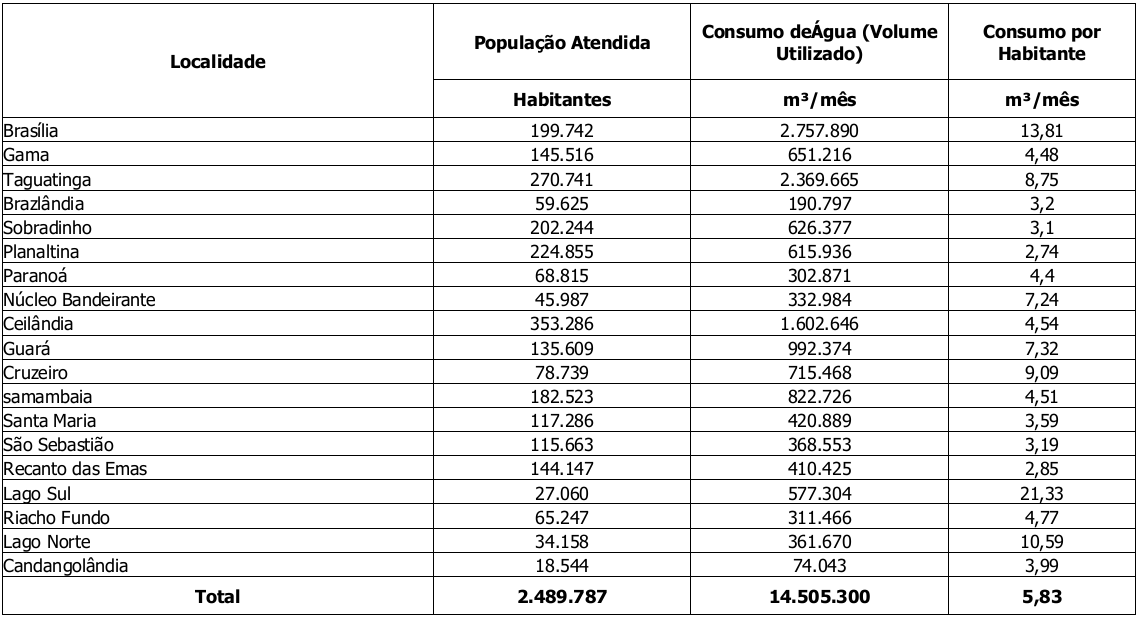
\includegraphics[keepaspectratio,scale=0.3]{figuras/table1.png}
\caption{Consumo médio de água \cite{table1}}

\end{figure}

\subsection{Por que reutilizar a água?}

	O reúso da água consiste simplesmente em se tentar reaproveitá-la depois que ela cumpriu sua função inicial, sendo necessário para isso, na maioria dos casos, um tratamento prévio que varia de complexidade dependendo do uso que dela foi feito.

	É claro que a primeira coisa a ser feita com relação à água é economizar. Diminuindo o consumo, dentro do possível, evitamos os gastos gerados com as iniciativas de reaproveitar a água. É o meio mais racional. Mas, quando não é mais possível diminuir o consumo, temos então que tentar reutilizá-la da melhor forma possível de forma que seja, também, economicamente viável e compensadora.

	Por se tratar de um bem natural que está cada vez mais raro e caro, 
reutilizar a água é de fundamental importância para o meio ambiente e também 
para a economia das empresas, cidadãos e governos.

Evitar o desperdício é a chave para a preservação. Se todos se colocarem a racionar e reutilizar então não faltará para ninguém.

\subsection{Qual água reutilizar? Como reutilizar?}

	O sistema de reuso de águas cinzas (expurgo de chuveiros, lavatórios, lavadoras de roupas, tanques), podendo ser conjugado com Aproveitamento de Água de Chuva. Sendo reutilizáveis em vasos sanitários, para lavar pisos e carros, irrigar plantas, enfim para uso geral de águas não potáveis. A proposta desse sistema se dá, após estudos quando ao índice pluviométrico do DF, no qual é muito baixo, para se considerar um reaproveitamento da água da chuva e o custo do maquinário necessário para torna-la potável. Como proposta, tem-se que a água proveniente da chuva e de descarte da casa, ela será aproveitada para outros fins, o que já reduzirá no consumo médio da água proveniente das centrais de abastecimento. Reduzindo custos a longo prazo e visando a empregabilidade do conceito de consciência sustentável.

\subsection{Como medir a relação produção/consumo dessa água?}

	Após o estabelecimento da rotina de cada morador na casa, é possível determinar quase com exatidão o seu consumo diário para assim poder fazer o cálculo do percentual de consumo hídrico e o que poderá ser reutilizável. Tais requisitos serão preenchidos posteriormente.

\section{Reutilização do Lixo}
\subsection{Qual tipo de lixo a família vai produzir?}

Uma família comum produz três tipos de lixo:
\begin{itemize}
	\item Orgânico (restos de comidas, matéria orgânica);
	\item Reciclável (matérias reutilizáveis, plásticos, metais, papeis, etc.);
	\item Esgoto (matéria não-reaproveitável);
\end{itemize}

	Apenas o lixo orgânico será reaproveitado para outros fins na residência, fazendo-se o uso de uma composteira residencial, afim de aproveitar a matéria orgânica decomposta para a adubação de jardins e hortas. Sendo de baixo custo e preocupação mínima com a manutenção, e podendo ser manuseada e “cuidada” por todos os integrantes da casa, sem requerer conhecimentos específicos ou aprofundados. 

\subsection{Quais vantagens de se reutilizar o lixo?}

	Solução eficaz para reciclagem de lixo orgânico, a compostagem doméstica é uma prática de múltiplos benefícios. Primeiro, pelo impacto positivo ao meio ambiente, ao reduzir em até 75\% o volume de resíduos orgânicos depositado nos aterros sanitários. Segundo, porque possibilita a fabricação de fertilizantes nutritivos para uso em hortas, vasos e jardins a custo zero.

\subsection{Como direcionar os produtos recicláveis?}

	Já a matéria reciclável será enviada às entidades e ONGs voltadas para a reutilização desse material.

\subsection{O que fazer com o esgoto produzido? Por quê?}

	Os dejetos não-reaproveitáveis serão descartados numa rede de esgoto da região, embora seja possível seu tratamento, para o reuso na residência. Porém esse processo necessita de cuidados e manutenções contínuas e de alto custo, além de uma mão-de-obra especializada. O que torna seu emprego inviável para a quantidade de resíduos produzidas pela família, que gera em torno dos 450 L diários.\cite{estimativaNBR7229}\cite{ecycle}
